% ==============================================================================
% Appendix: Statistical Details
% ==============================================================================

\section{Statistical Appendix}
\label{sec:appendix_stats}

\subsection{Autocorrelation Assessment}

XRF measurements at 3~mm intervals share depositional and diagenetic history with their neighbors. Table~\ref{tab:autocorrelation_appendix} shows lag-1 autocorrelation coefficients for primary proxies, confirming that individual measurements cannot be treated as independent samples \citep{Hurlbert1984}.

\begin{table}[h]
\centering
\caption{Lag-1 autocorrelation coefficients}
\label{tab:autocorrelation_appendix}
\begin{tabular}{lrrr}
\toprule
Site & Fe/Mn & Ca & Ti \\
\midrule
TAM & 0.70 & 0.70 & 0.67 \\
SC & 0.81 & 0.67 & 0.55 \\
\bottomrule
\end{tabular}
\end{table}

\subsection{Multi-Proxy Comparison}

Figure~\ref{fig:multiproxy_appendix} shows section-level distributions for four geochemical proxies. Only Fe/Mn shows a significant difference after Bonferroni correction ($\alpha$ = 0.006 for 8 tests). Ti, Zr/Rb, and Ca/Ti show moderate effects in the expected directions but do not reach statistical significance.

\begin{figure}[h]
\centering
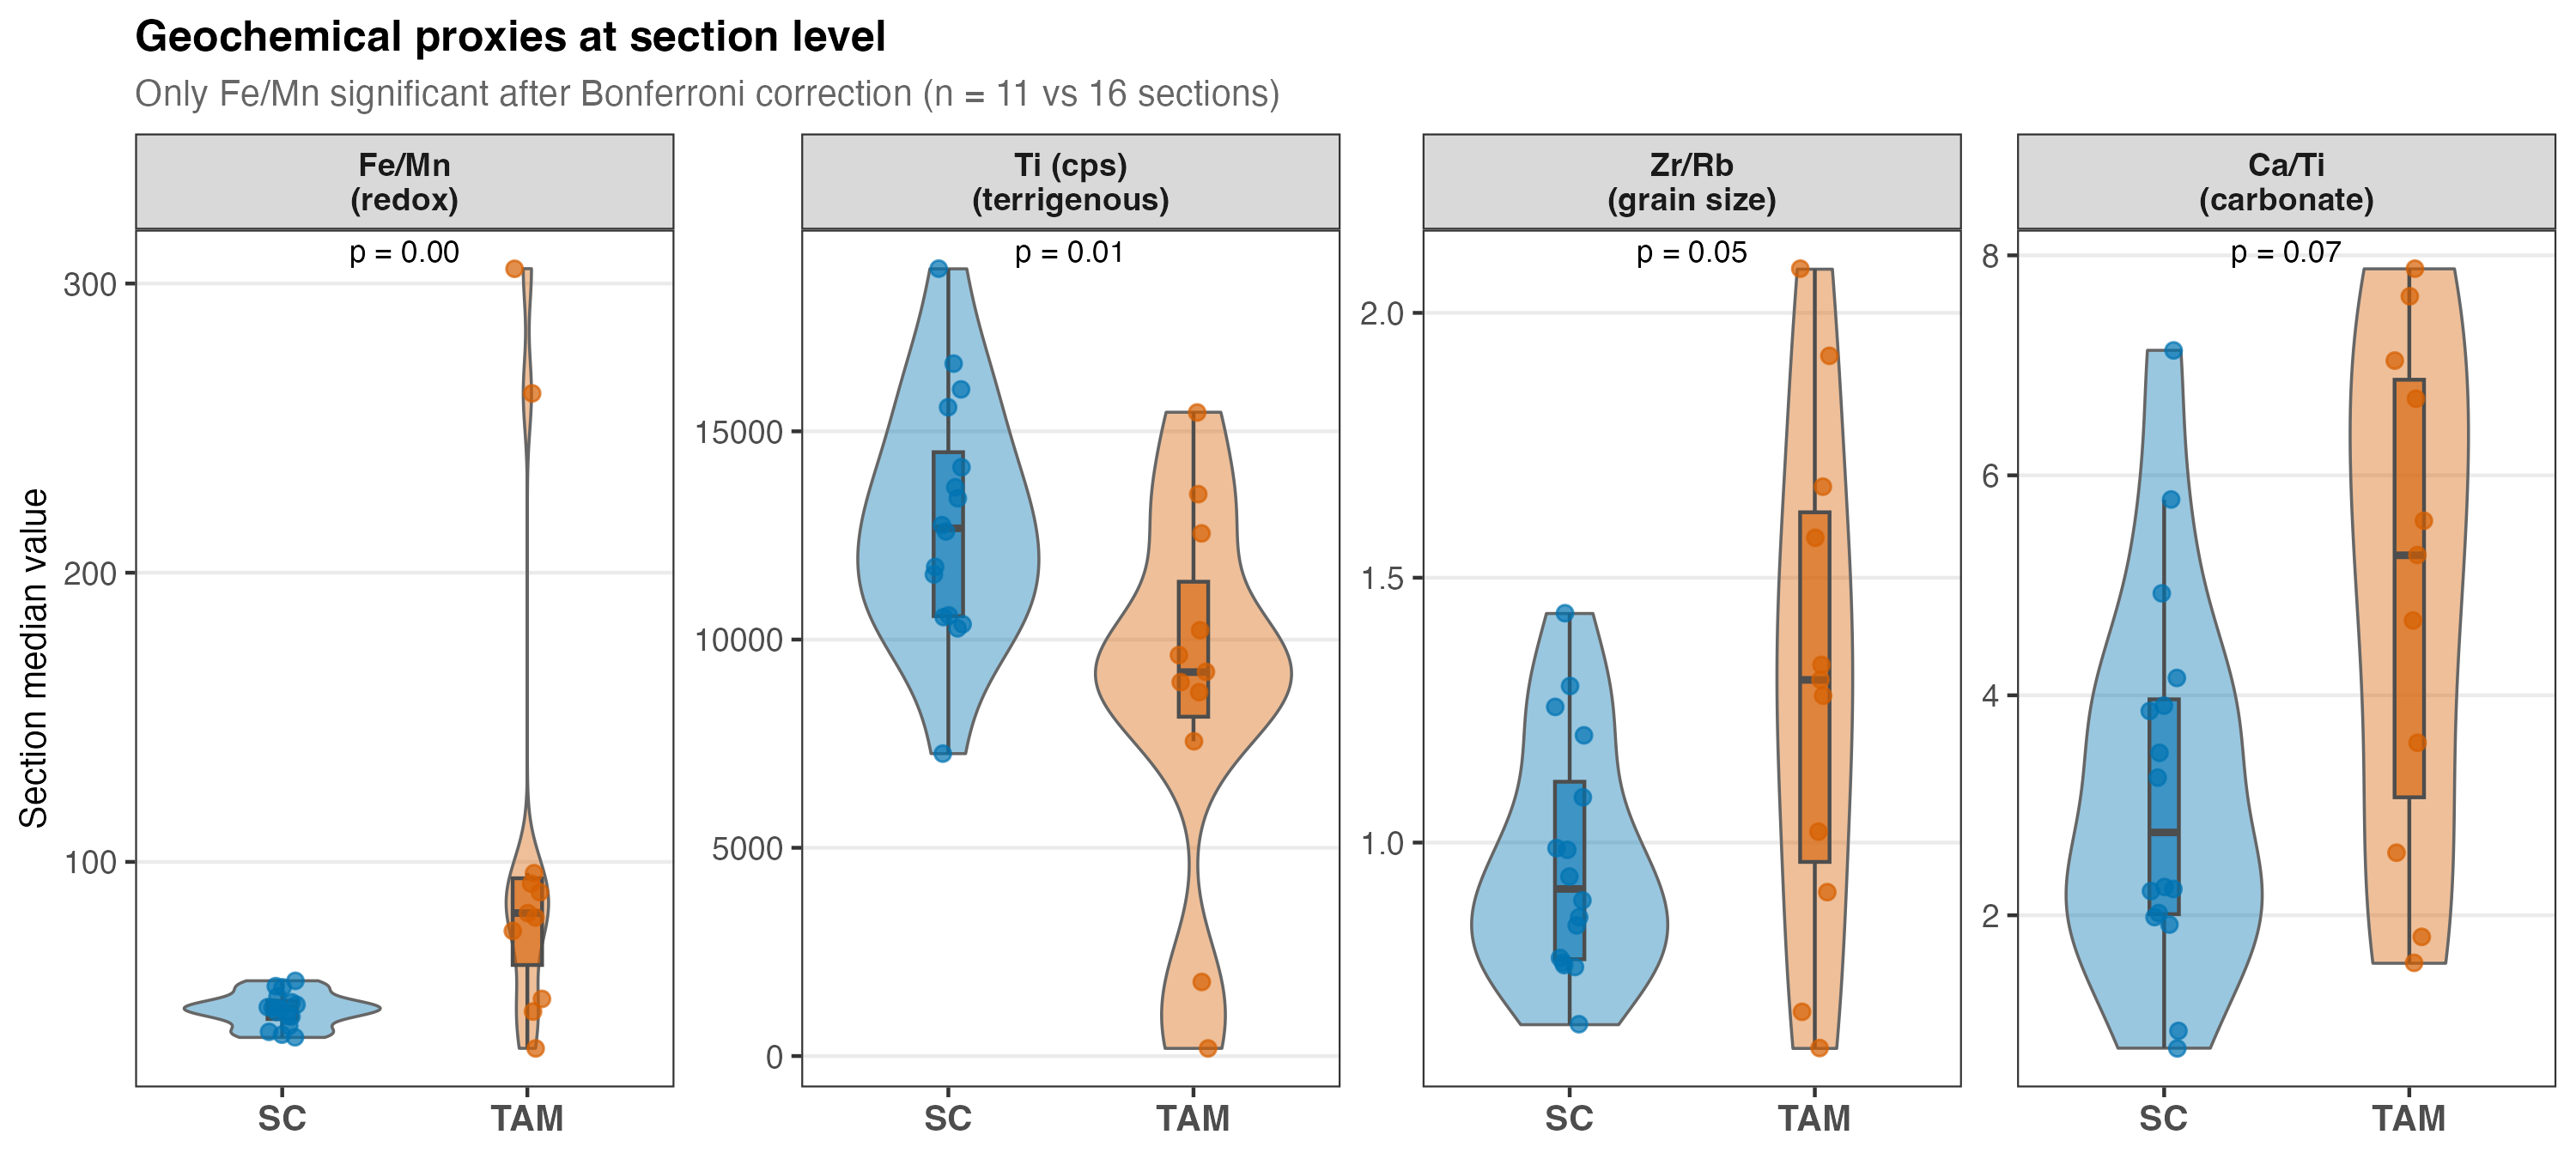
\includegraphics[width=\textwidth]{figures/site_comparison/fig_violin_multiproxy.png}
\caption{Geochemical proxies at section level. Each point represents one core section ($n$ = 11 TAM, 16 SC). Only Fe/Mn is significant after multiple comparison correction.}
\label{fig:multiproxy_appendix}
\end{figure}

\subsection{Effect Sizes}

Figure~\ref{fig:effect_appendix} shows Cliff's delta effect sizes for all proxies tested. Values exceeding $\pm$0.47 indicate large effects. Fe/Mn and its derived measure (\% reducing) show large effects; other proxies show small to moderate effects.

\begin{figure}[h]
\centering
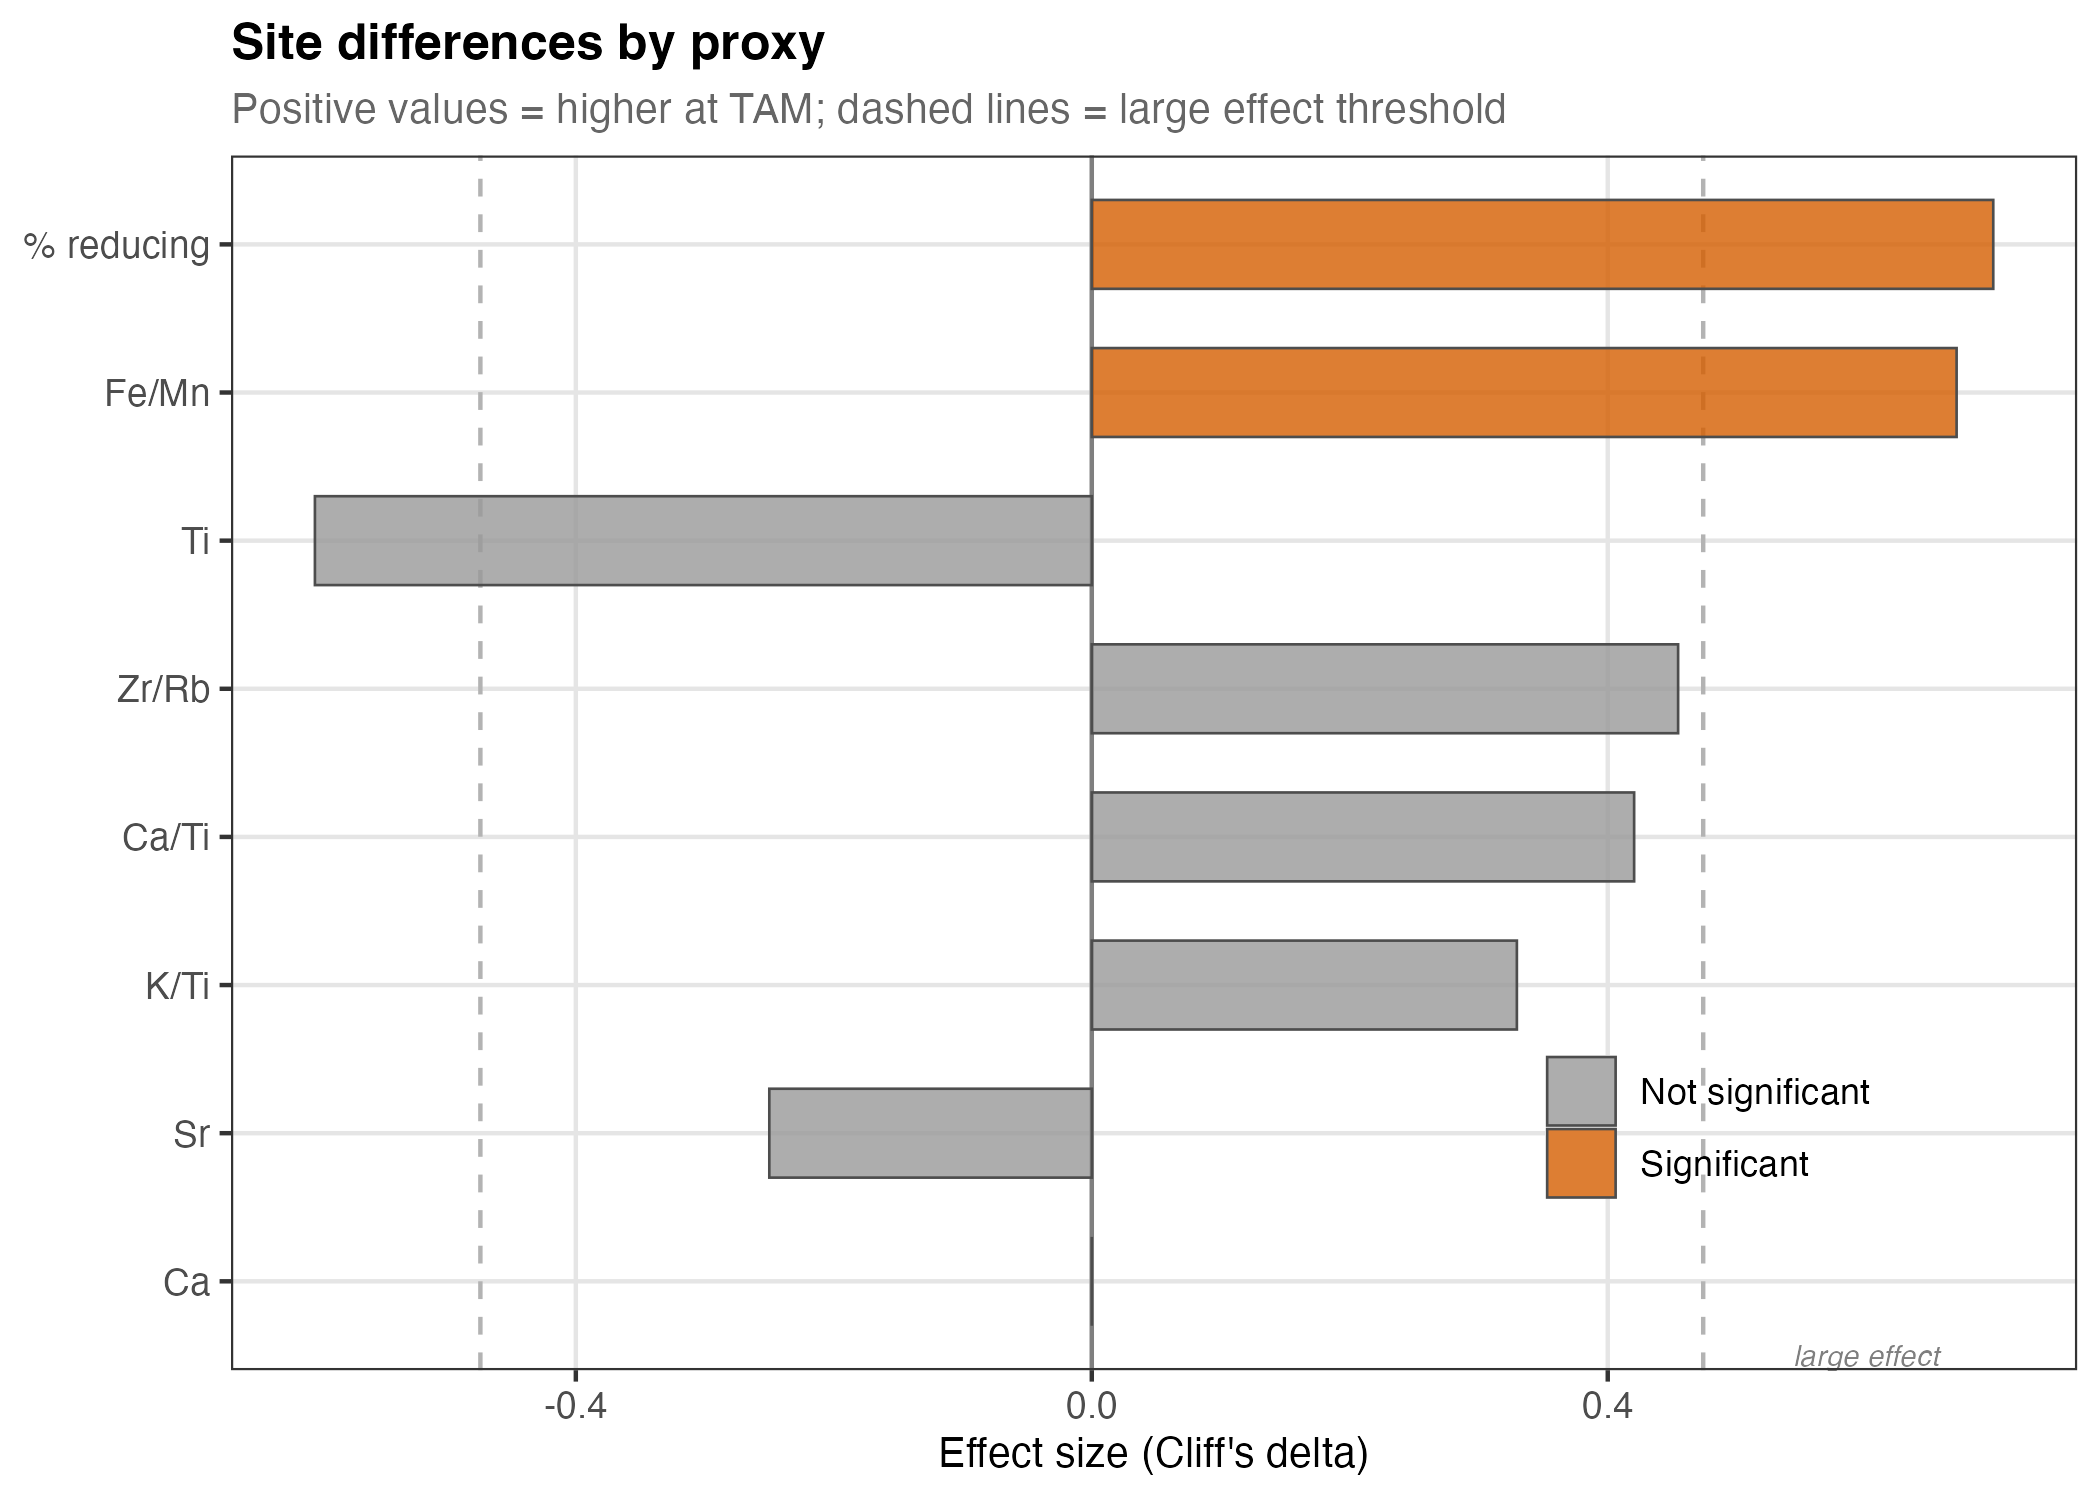
\includegraphics[width=0.8\textwidth]{figures/site_comparison/fig_effect_sizes.png}
\caption{Effect sizes (Cliff's delta) for site comparisons. Positive values indicate higher values at TAM. Dashed lines mark the large effect threshold.}
\label{fig:effect_appendix}
\end{figure}

\subsection{Stratigraphic Profiles}

Figure~\ref{fig:strat_appendix} shows representative Fe/Mn profiles from each site, illustrating within-core variability. The TAM section remains predominantly above the reducing threshold, while the SC section oscillates around it.

\begin{figure}[h]
\centering
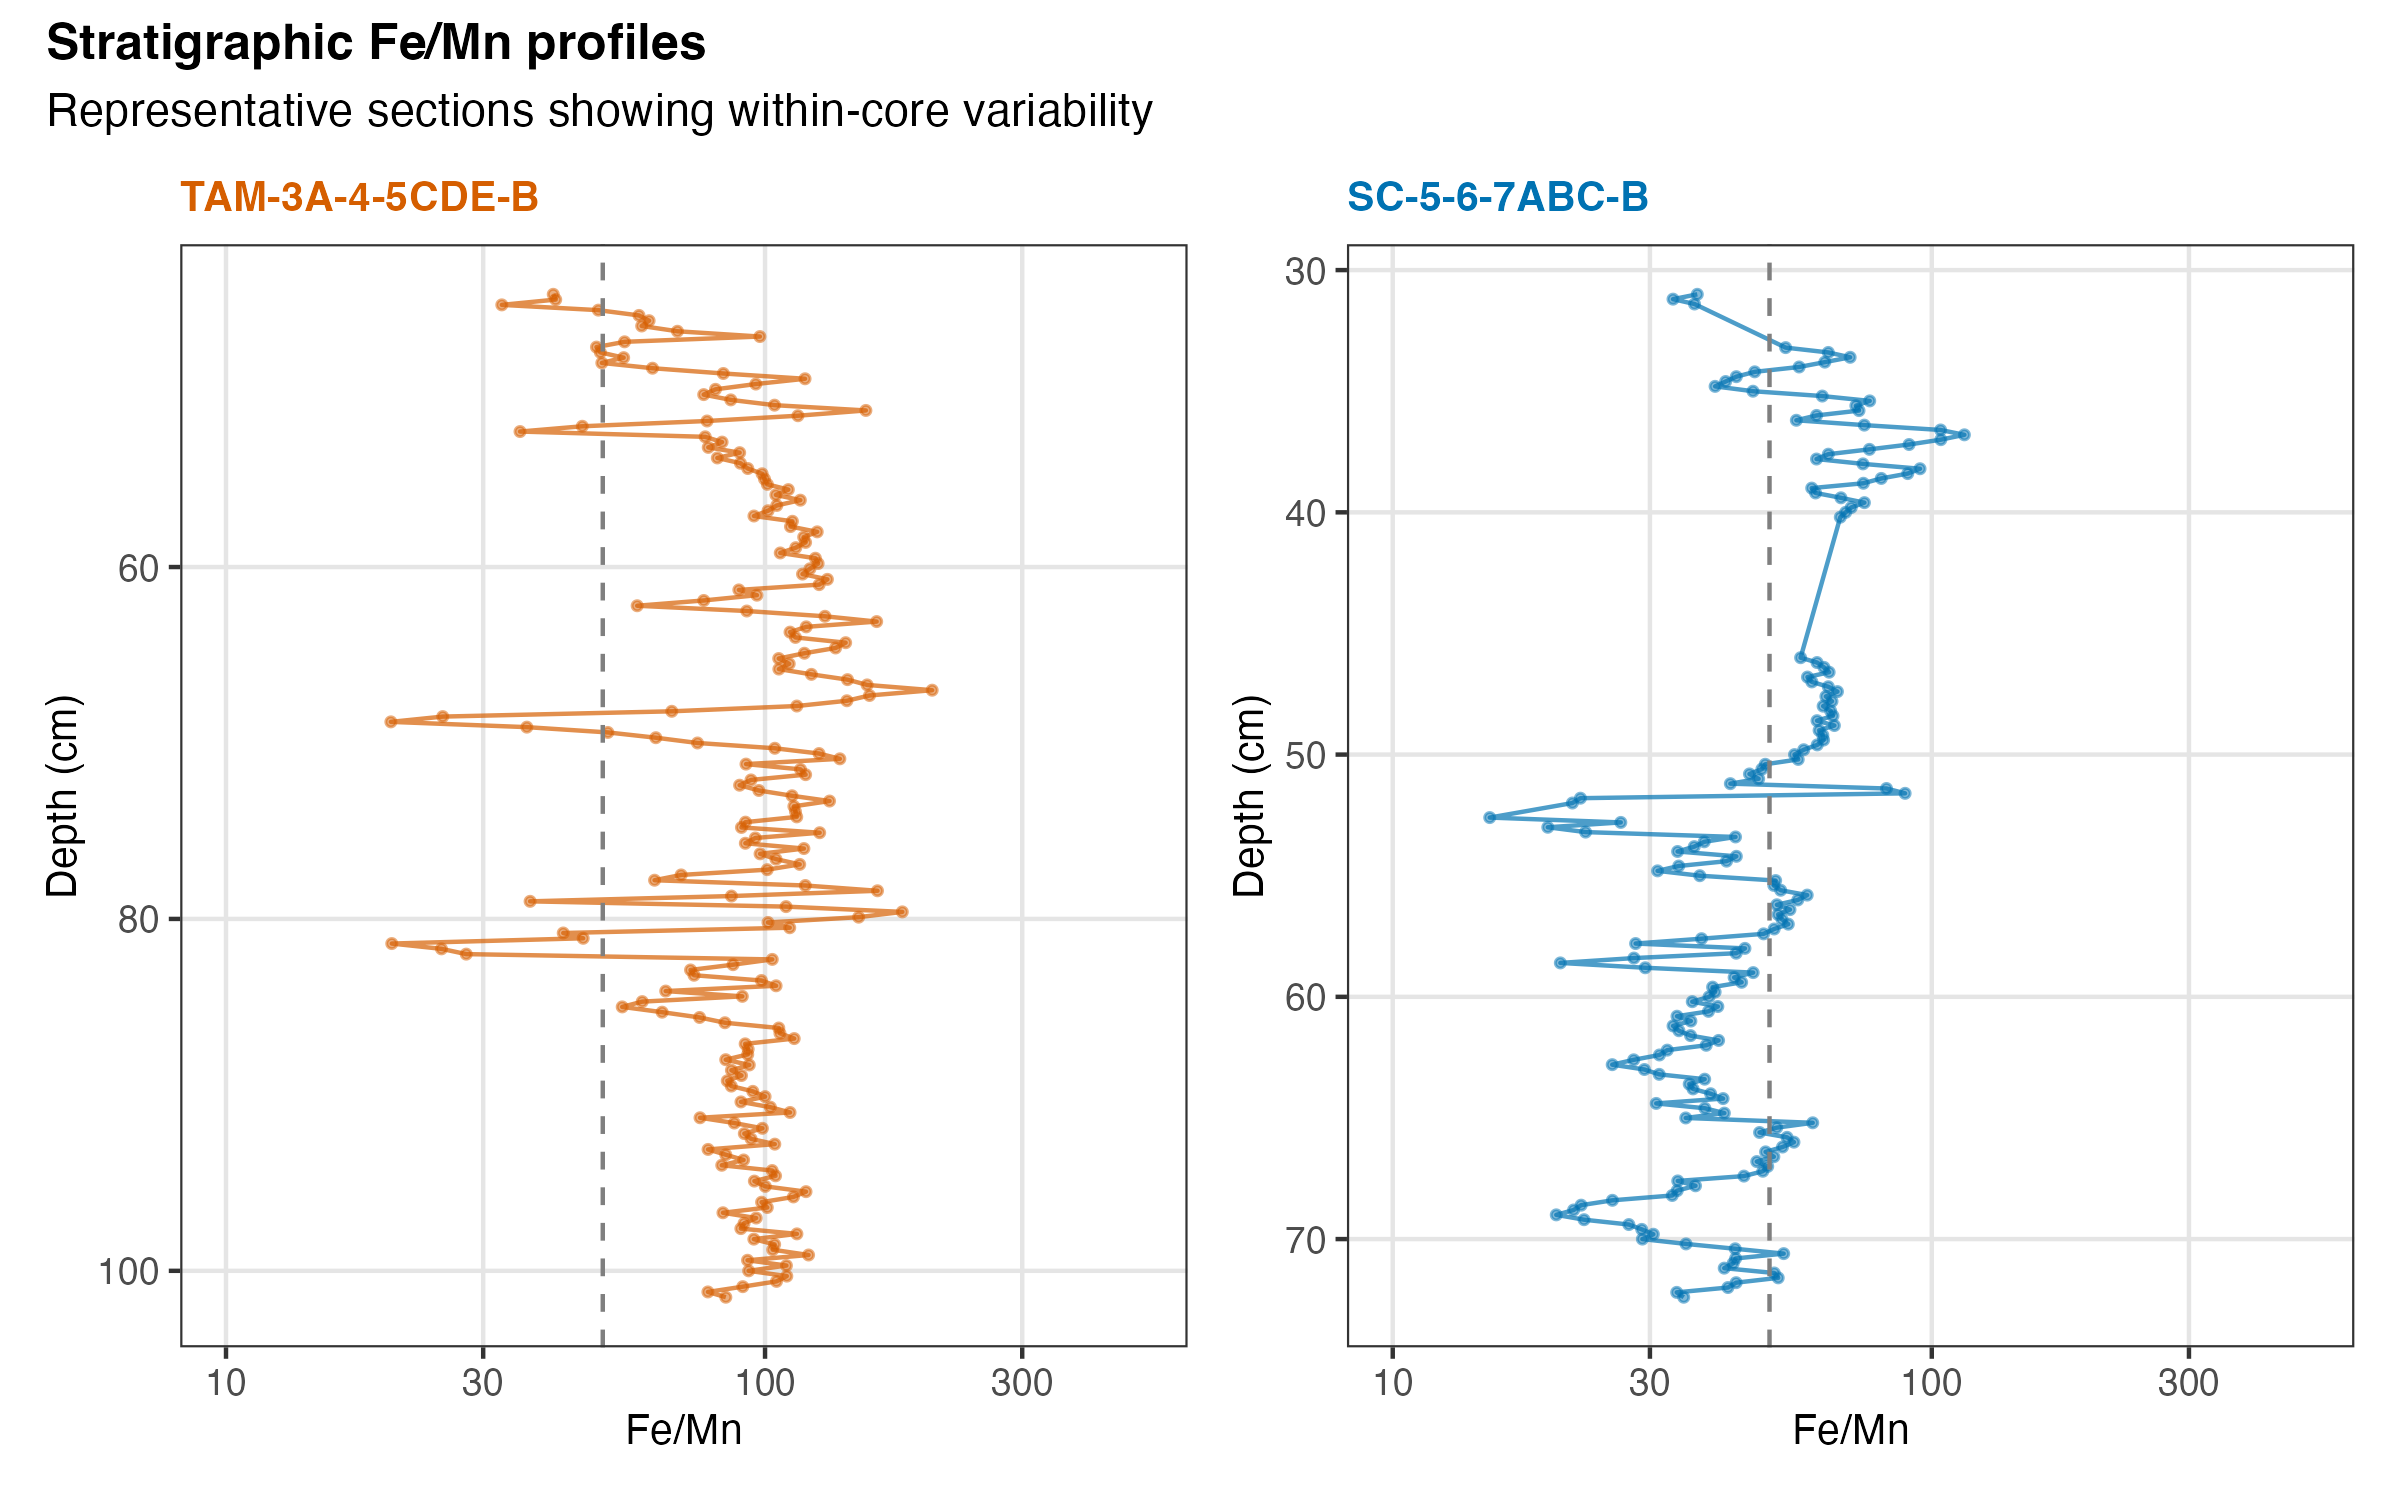
\includegraphics[width=\textwidth]{figures/site_comparison/fig_stratigraphic_profiles.png}
\caption{Representative Fe/Mn downcore profiles. Dashed line marks Fe/Mn = 50 (reducing threshold).}
\label{fig:strat_appendix}
\end{figure}

\subsection{Spectral Analysis}
\label{sec:appendix_spectral}

To test for cyclic variability, we analyzed the Fe/Mn profile from the longest continuous section (TAM-3A-4-5CDE-B, 191 measurements) using FFT spectral analysis with AR(1) red noise significance testing.

Apparent periodicities at wavelengths of $\sim$40~cm and $\sim$95~cm are present in the power spectrum, but these do not exceed the 95\% confidence level against a red noise null hypothesis (Figure~\ref{fig:spectral_appendix}). Without independent age control, we cannot interpret depth-domain features as evidence for orbital forcing.

\begin{figure}[h]
\centering
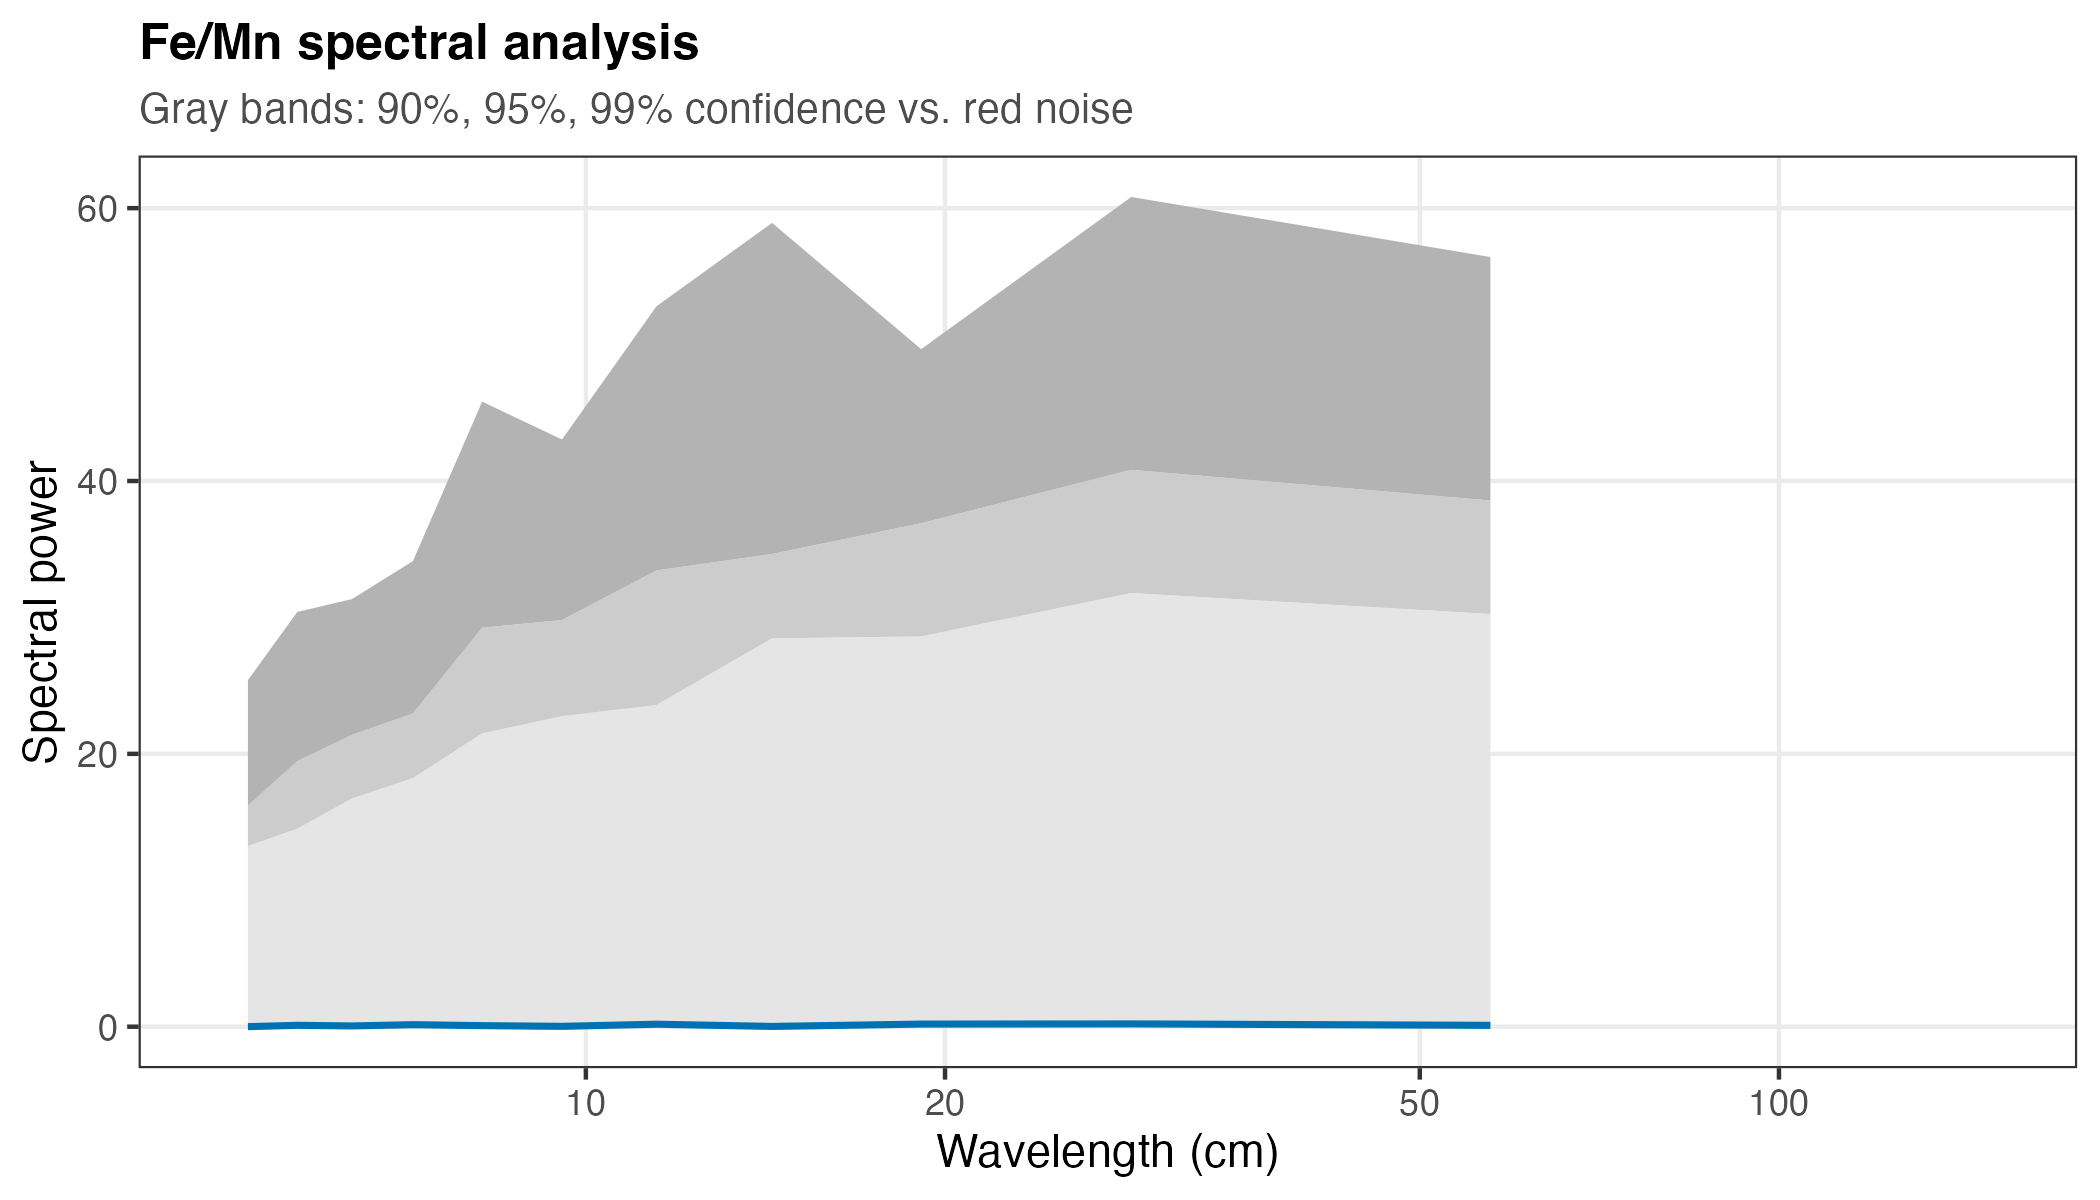
\includegraphics[width=0.8\textwidth]{figures/site_comparison/fig_stat_4_spectral_significance.png}
\caption{Spectral analysis of Fe/Mn. Gray shading shows 90--99\% confidence bounds from AR(1) red noise simulations. No peaks exceed the 95\% level.}
\label{fig:spectral_appendix}
\end{figure}

\subsection{Fe-Mn Decoupling}

The weaker correlation between Fe and Mn at TAM ($r$ = 0.18) compared to SC ($r$ = 0.67) is consistent with redox-driven fractionation. Under reducing conditions, Mn is mobilized preferentially to Fe, decoupling their otherwise coherent terrigenous signal.

\begin{figure}[h]
\centering
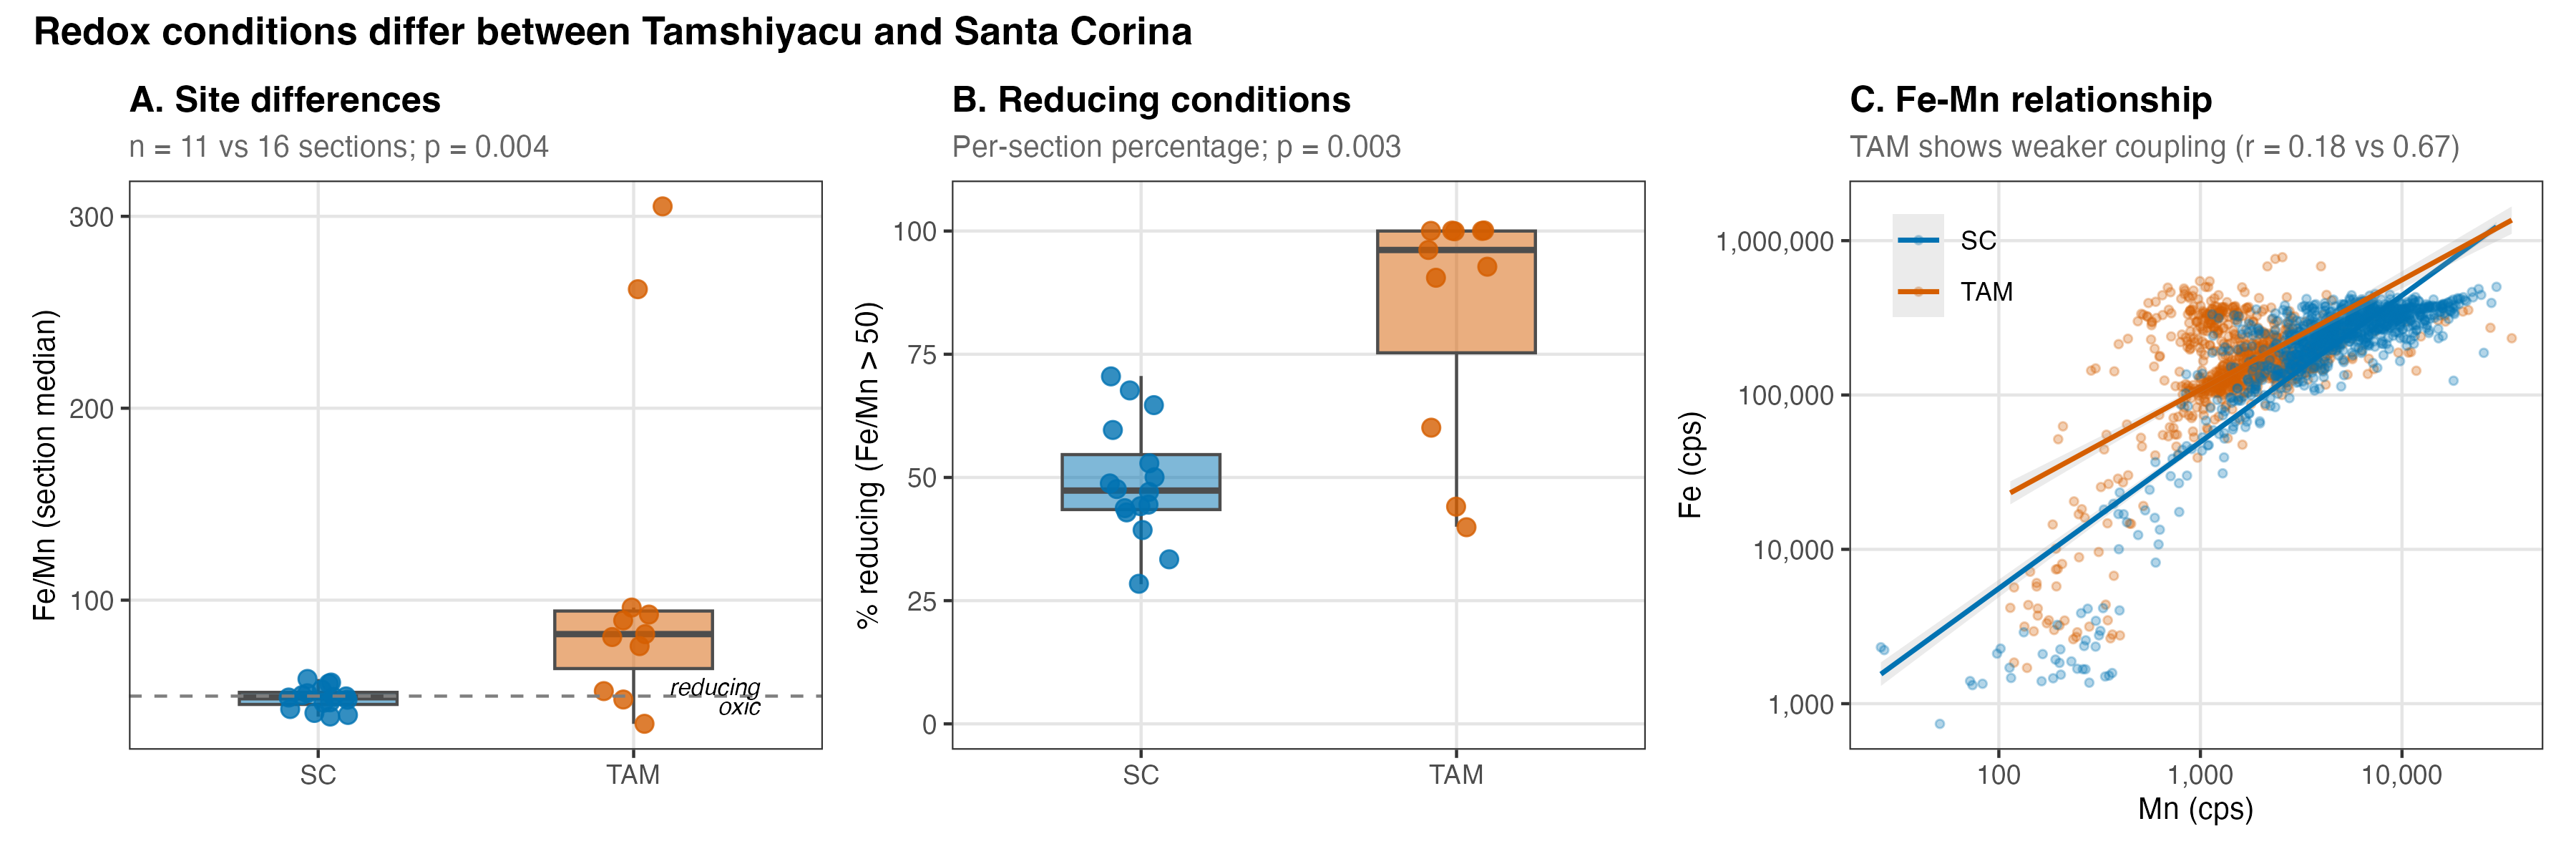
\includegraphics[width=0.7\textwidth]{figures/site_comparison/fig_redox_comparison.png}
\caption{Three views of the TAM-SC redox difference. (A) Section-level Fe/Mn medians. (B) Percentage of reducing conditions per section. (C) Fe-Mn relationship showing weaker coupling at TAM.}
\label{fig:redox_appendix}
\end{figure}
